\begin{ledgroupsized}[r]{120mm}
\footnotesize 
\pstart 
\noindent\textbf{\"{U}berlieferung:}
\pend
\end{ledgroupsized}
\begin{ledgroupsized}[r]{114mm}
\footnotesize 
\pstart \parindent -6mm
\makebox[6mm][l]{\textit{L}}Konzept: LH XXXVII 5 Bl. 215. 1 Bl. 4\textsuperscript{o}. 1 S. auf Bl. 215~r\textsuperscript{o}. Bl. 215~v\textsuperscript{o} leer.
Textträger durch Papiererhaltungsmaßnahmen stabilisiert.\\
Cc 2, Nr. 835
\pend
\end{ledgroupsized}
%
\vspace*{8mm}%
\count\Afootins=1200
\count\Bfootins=1200
\count\Cfootins=1200
\pstart%
\normalsize%
\noindent%
% [215~r\textsuperscript{o}]
[215~r\textsuperscript{o}] Xb: 1674
\pend
\vspace*{0.5em}% PR: Rein provisorisch !!!
\pstart% PR: Bitte als Überschrift setzen.
\centering%
\noindent%
% \begin{center}%
De vitandis erroribus Geometricis in re mechanica
% \end{center}
% \pstart%
% \noindent%
% \hangindent=15mm%
% Imo recte.
\pend
\vspace*{0.5em}% PR: Rein provisorisch !!!
\pstart%
\noindent%
\hangindent=7,5mm%
(1)\hspace{1.2mm}
\edtext{Error\edtext{}{\lemma{}\Afootnote{\textit{Über dem Zeilenanfang:} Imo recte.\vspace{-4mm}}}
P. Pardies,\protect\index{Namensregister}{Pardies, Ignace Gaston SJ (1636-1673)}
qui ait (inspice \edtext{fig. 1) vires ponderum\protect\index{Sachverzeichnis}{vires ponderum} $B$, et $C$ esse}{\lemma{fig. 1.)}\Bfootnote{\textit{(1)} vim ponderis $B$, esse ad vim ponde \textit{(2)} vires ponderum $B$, et $C$ esse \textit{L}}} in composita ratione rectarum $AB$, $AD$ et ipsorum ponderum.
Generalem enim condit regulam brachium librae\protect\index{Sachverzeichnis}{brachium librae}
aestimandum esse \edtext{longitudine perpendicularis $AD$}{\lemma{longitudine}\Bfootnote{\textit{(1)} rectae \textit{(2)} perpendicularis $AD$ \textit{L}}}
ex centro ut $A,$ ad lineam directionis $ED$ ducto.%
}{\lemma{Error [...] ducto}\Cfootnote{\cite{01092}\textsc{I.G. Pardies}, \textit{La statique}, 2. Ausg., Paris 1674, Kap. XXXII, S. 42-44.}}
Sed mihi nec regula illa certa videtur, certe non demonstrat, nec ipsa $ED$ appellari debere linea directionis.
\pend
\vspace*{1.5em}
\pstart
\centering
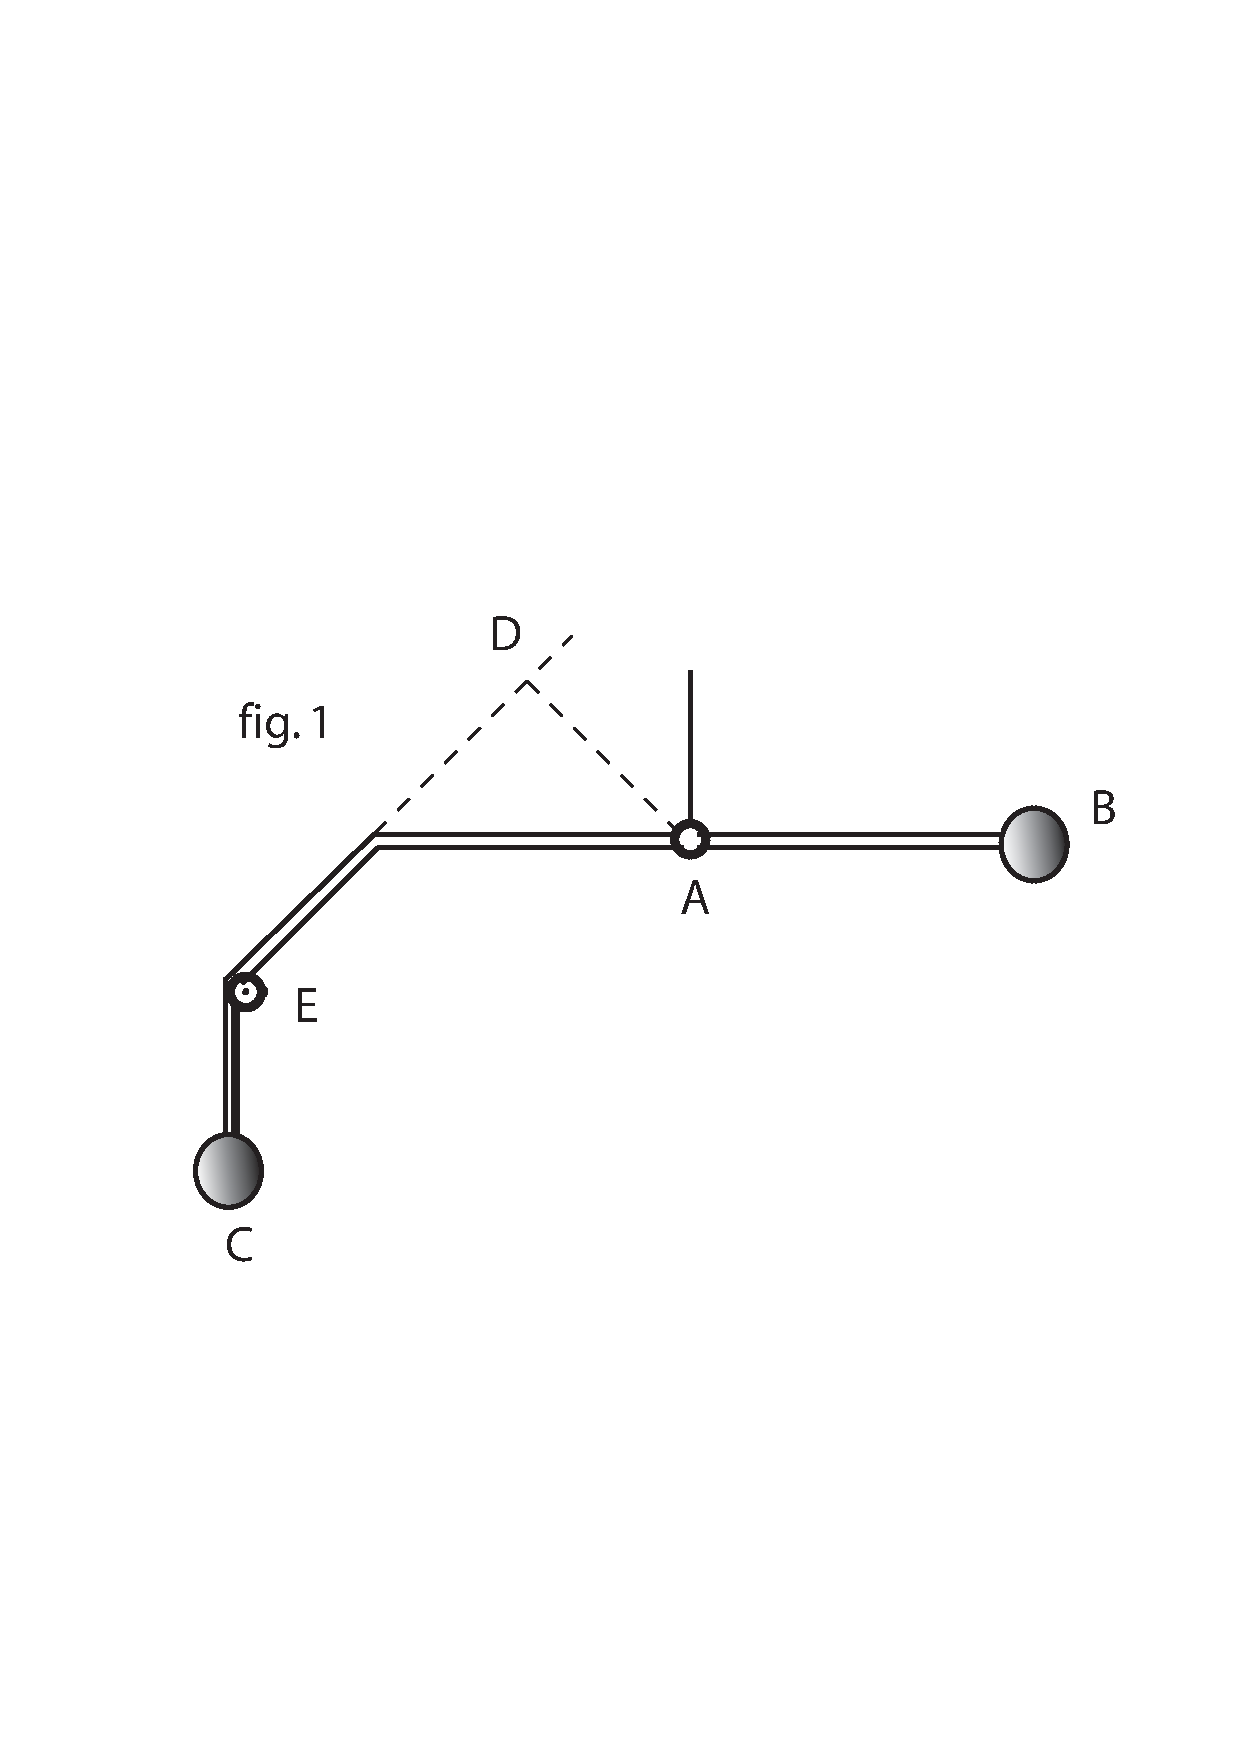
\includegraphics[width=0.53\textwidth]{images/LH03705_215r-d1.pdf}
\pend
\newpage
\count\Bfootins=1200
\count\Cfootins=1200
\pstart
\centering
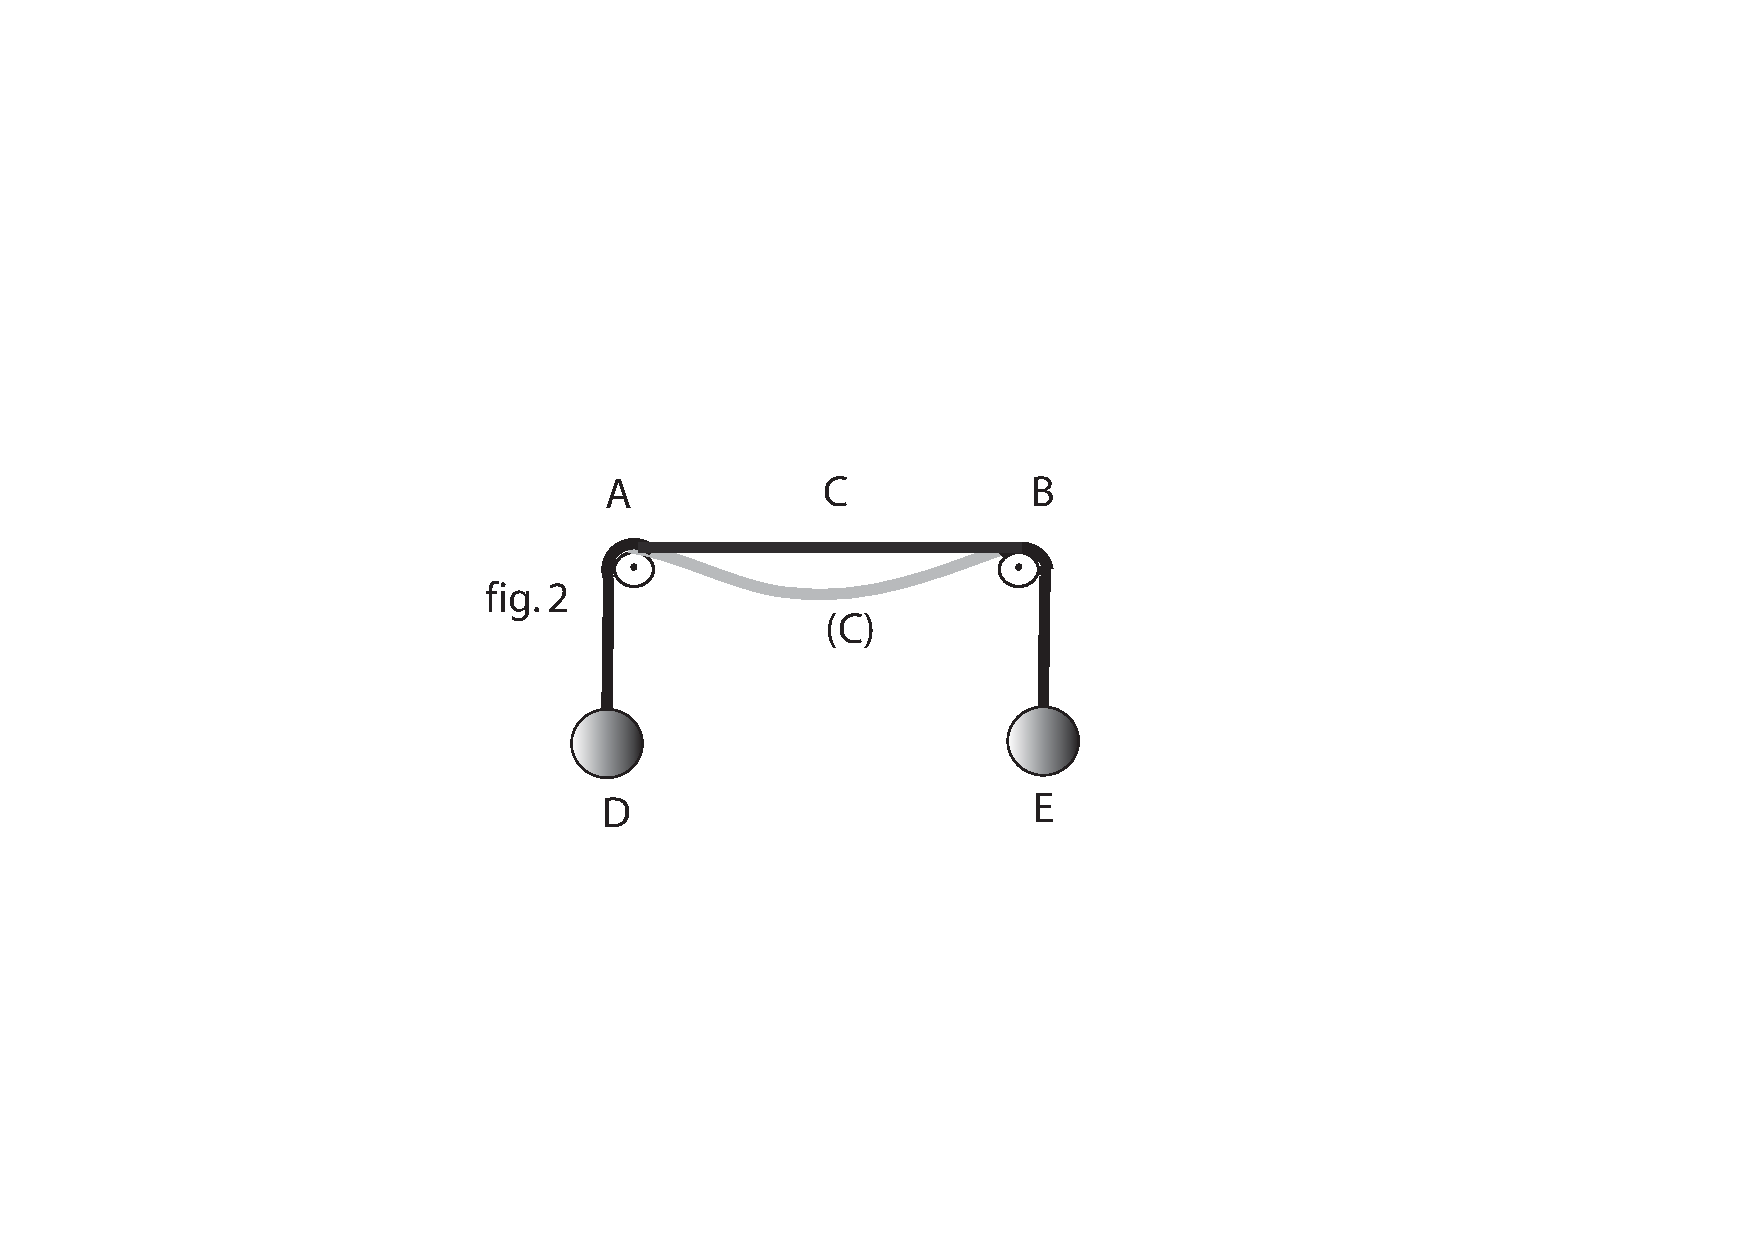
\includegraphics[width=0.38\textwidth]{images/LH03705_215r-d2.pdf}
%\lbrack\textit{Fig. 1 und 2}\rbrack
%\rule[0pt]{20mm}{0pt}
\pend
\vspace*{1.5em}
\pstart%
\noindent%
\setline{1}
\hangindent=7,5mm%
(2)\textso{ }%
\edtext{\textso{Error ejusdem.} Hinc autem ducit consequentiam, quod chorda nulla vi perfecte tendi possit. Nam esto \edtext{chorda $ACB$ per trochleas\protect\index{Sachverzeichnis}{trochleas} $A$, $B$, transiens}{\lemma{chorda $ACB$}\Bfootnote{\textit{(1)} trochleis $A$, $B$, circumplicata \textit{(2)} per trochleas $A$, $B$, transiens \textit{L}}}, tensa ponderibus $D$, $E$; ait eam nunquam perfecte \edtext{tensam fore}{\lemma{tensam}\Bfootnote{\textit{(1)} esse \textit{(2)} fore \textit{L}}} quantacunque sit vis ponderum, sed loco \edtext{situs perfecte tensi}{\lemma{situs}\Bfootnote{\textit{(1)} recte \textit{(2)} perfecte tensi \textit{L}}} $ACB$, semper fore in semilaxo $A(C)B$ quod cum manifeste rationi adversum sit; nam necesse est hoc modo pondus\protect\index{Sachverzeichnis}{pondus} chordae $C$ praevalere \edtext{ponderibus $D$, $E$, quod est contra hypothesin}{\lemma{ponderibus $D$, $E$,}\Bfootnote{\textit{(1)} nam cum tendi \textit{(2)} at certe augeri \textit{(3)} est \textit{(4)} quod est contra hypothesin. \textit{L}}}.%
}{\lemma{\textso{Error} [...] hypothesin}\Cfootnote{\cite{01092}a.a.O., Kap. LXIX, S. 118f.}}
At si pondera praevalent non video cur non amplius attrahant. Neque enim video quo colore dici possit chordam machinae cujusdam hoc loco habere naturam qua magna a parvis elevantur.
\pend
\pstart%
\noindent%
\hangindent=7,5mm%
(3)\hspace{1mm}
\edtext{Error Clarissimi Regnaldi\protect\index{Namensregister}{\textso{Regnauld} (Regnaldus), Fran\c{c}ois 1689} circa dimensiones \edtext{superficierum sphaeroeidum insertus est Itinerario Monconisii,\cite{00118}\protect\index{Namensregister}{\textso{Monconys} (Monconisius), Balthasar de 1611-1665} part. 3.}{\lemma{superficierum}\Bfootnote{\textit{(1)} curvarum Elli \textit{(2)} sphaeroeidum \textit{(a)} inserta est dimensio \textit{(b)} inserta est ea dimensio \textit{(c)} insertus est Itinerario Monconisii, part. 3. \textit{L}}}%
}{\lemma{Error [...] part. 3}\Cfootnote{\cite{00118}\textsc{B. de Monconys}, \textit{Journal des voyages}, Bd. III, Lyon 1666, S. 15-24.}}
Videtur ibi abusus methodo indivisibilium.
\edtext{Qua occasione \edtext{adjectus error R. P. Fabri in demetienda curva Ellipseos.%
}{\lemma{adjectus [...] Ellipseos}\Cfootnote{\cite{00335}\textsc{H. Fabri}, \textit{Synopsis geometrica}, Lyon 1669, S. 285f. Siehe hierzu \textit{LSB} VII, 4 \cite{01093}N. 1, S. 18; ebd. \cite{01094}N. 11, S. 167 und 170.}}%
}{\lemma{}\Bfootnote{Qua occasione [...] curva Ellipseos. \textit{erg. L}}}
\pend
\pstart%
\noindent%
\hangindent=7,5mm%
(4)\hspace{1mm}
\edtext{Error Clarissimi cujusdam Geometrae (:~id est Robervallii~:)\protect\index{Namensregister}{\textso{de Roberval}, Gilles Personne 1602-1675}
circa vires vectis\protect\index{Sachverzeichnis}{vires compositi} compositi,%
}{\lemma{Error [...] compositi}\Cfootnote{\cite{00504}\textsc{G. de Roberval}, \textit{Traité de Méchanique}, Paris 1636, S. 21ff.}}
inspice figuram 3.
\edtext{Demonstrati sunt a me casus omnes;
etiam cum centra duorum vectium non sunt in una horizontali;
et in eam rem \edtext{dedi regulam generalem}{\lemma{dedi}\Bfootnote{\textit{(1)} theorema generale \textit{(2)} regulam generalem \textit{L}}}
omnes casus complexam, quae constructione geometrica absolvitur.%
}{\lemma{Demonstrati [...] absolvitur}\Cfootnote{Vermutlich Anspielung auf N.~45.}}
%Demonstrati sunt a me casus omnes;
%etiam cum centra duorum vectium non sunt in una horizontali;
%et in eam rem \edtext{dedi regulam generalem}{\lemma{dedi}\Bfootnote{\textit{(1)} theorema generale \textit{(2)} regulam generalem \textit{L}}}
%omnes casus complexam, quae constructione geometrica absolvitur.
Clarissimus \edtext{Romerus\protect\index{Namensregister}{\textso{R{\o}mer}, Ole 1644-1710} Danus, iuvenis in Geometria inprimis et Astronomia versatissimus rem longius provexit, invenitque figuram quae dentibus rotarum danda sit, ut aequali semper vi agant; esse speciem cycloeidis secundariae, quae describitur rotatione circuli non in plano, sed \edtext{super acie cujusdam circuli.}{\lemma{super}\Bfootnote{\textit{(1)} acie \textit{(2)} quodam cylindro \textit{(3)} acie cujusdam circuli \textit{L}}}%
}{\lemma{Romerus [...] cujusdam circuli}\Cfootnote{Rømers Zahnräder wurden erst in seiner 1735 in Kopenhagen ver\-öf\-fent\-lich\-ten \cite{01096}\textit{Basis astronomiae} dargestellt. Folglich dürfte sich Leibniz hier vielmehr auf seinen persönlichen Austausch mit Rømer bzw. mit Huygens beziehen; siehe hierzu \cite{01095}seinen Brief an Johann Bernoulli vom 18. Januar 1698, \textit{LSB} III, 7 N. 178, S. 729.16-730.3. Zu beachten ist auch, dass ein Jahr später (im Dezember 1675) Leibniz ein Manuskript Rømers exzerpiert hat, welches ausdrücklich \textit{Propositiones mechanicae circa rotas dentatas} überlieferte. Siehe N. 98.% 037,05_216
}}
\pend 
\count\Bfootins=1200
\count\Cfootins=1200
%\begin{wrapfigure}{l}{0.3\textwidth}
%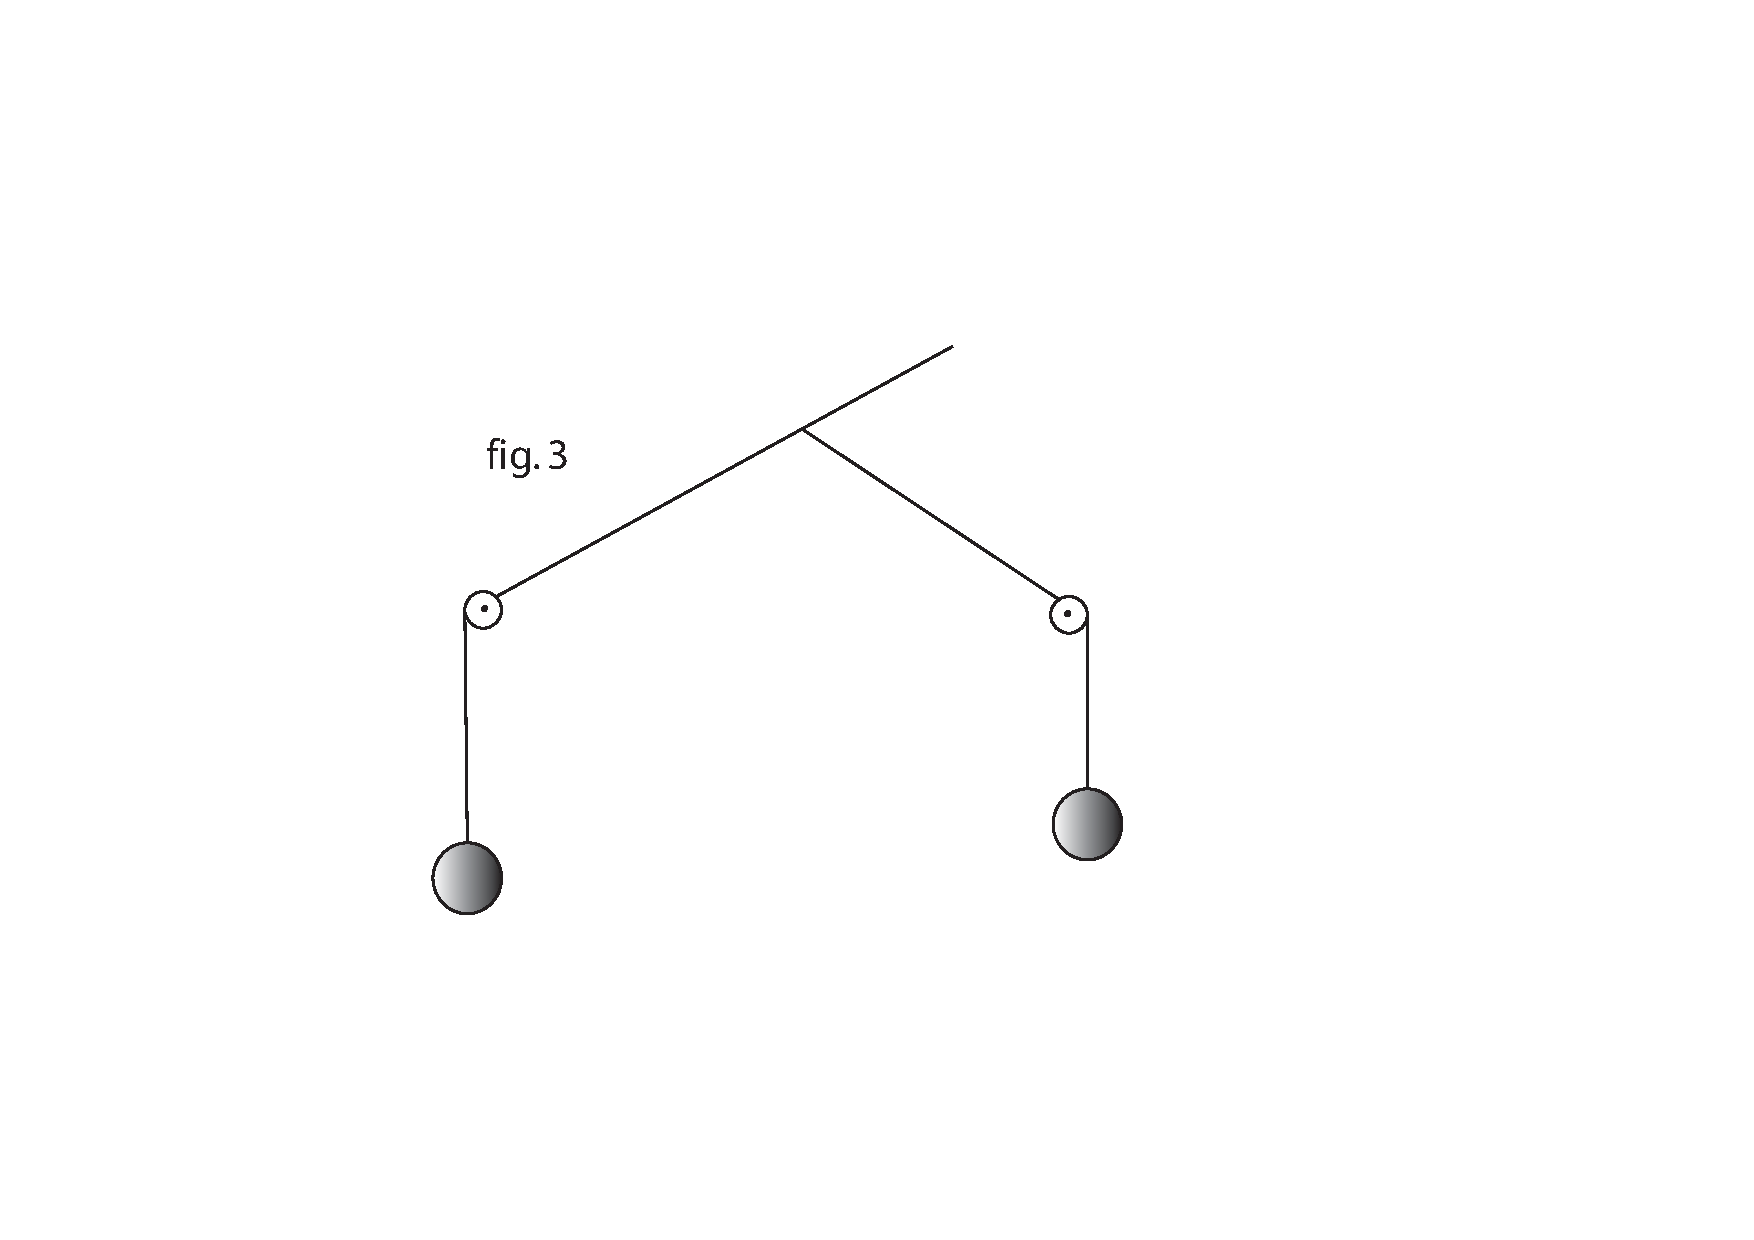
\includegraphics[width=0.3\textwidth]{images/LH03705_215r-d3.pdf}\\
%\rule[0pt]{20mm}{0pt}[\textit{Fig. 3}]
%\end{wrapfigure}
\pstart%
\noindent%
\hangindent=7,5mm%
(5)\hspace{1mm}
\edtext{De summi viri, Galilaei\protect\index{Namensregister}{\textso{Galilei} (Galilaeus, Galileus), Galileo 1564-1642} Paroramate, circa resistentiam solidorum.
Credidit ille parabolam aequalis ubique resistentiae\protect\index{Sachverzeichnis}{resistentia} esse.%
}{\lemma{De summi [...] esse}\Cfootnote{\cite{00050}\textsc{G. Galilei}, \textit{Discorsi}, Leiden 1638, S. 137-141 (\cite{00048}\textit{GO} VIII, S.~177-181).
Siehe hierzu N. 22.% F/4 = 037,05_209
}}
\edlabel{037,05_215_ref.1}%
Sed \edtext{Alexander de Marchettis\protect\index{Namensregister}{\textso{Marchetti} (de Marchettis), Alessandro 1633-1714} jam olim ait demonstrationem suam de Ellipsi amicis communicatam.%
}{\lemma{Alexander [...] communicatam}\Cfootnote{\cite{00336}\textsc{A. Marchetti}, \textit{De resistentia solidorum}, Flo\-renz 1669.
Vgl. dazu \cite{00506}\textsc{A. Favaro}, \textit{Amici e corrispondenti di Galileo}, Flo\-renz 1983, Bd. II, S. 1102-1106.}}
Sed et \edtext{Blondellus\protect\index{Namensregister}{\textso{Blondel} (Blondellus), Fran\c{c}ois 1618-1686}
Epistola ad Paulum W\"{u}rzium\protect\index{Namensregister}{\textso{W\''{u}rz} (Wurtz, Wurzius), Paul von 1612-1676} tunc Suecicarum copiarum
\edtext{ductorem, monitus}{\lemma{ductorem,}\Bfootnote{\textit{(1)} quam \textit{(2)} monitus \textit{L}}}
ab eo Galilaei\protect\index{Namensregister}{\textso{Galilei} (Galilaeus, Galileus), Galileo 1564-1642} sententiam.}{\lemma{Blondellus [...] sententiam}\Cfootnote{\cite{00337}\textsc{F. Blondel}, \textit{Epistola ad P.W.}, Paris 1661.}}
\edlabel{037,05_215_ref.2}%
De ruptura\protect\index{Sachverzeichnis}{ruptura} trabium inclinatarum, eadem occasione.
\pend
\vspace{2.5em}
\pstart
\advanceline{2}
\centering
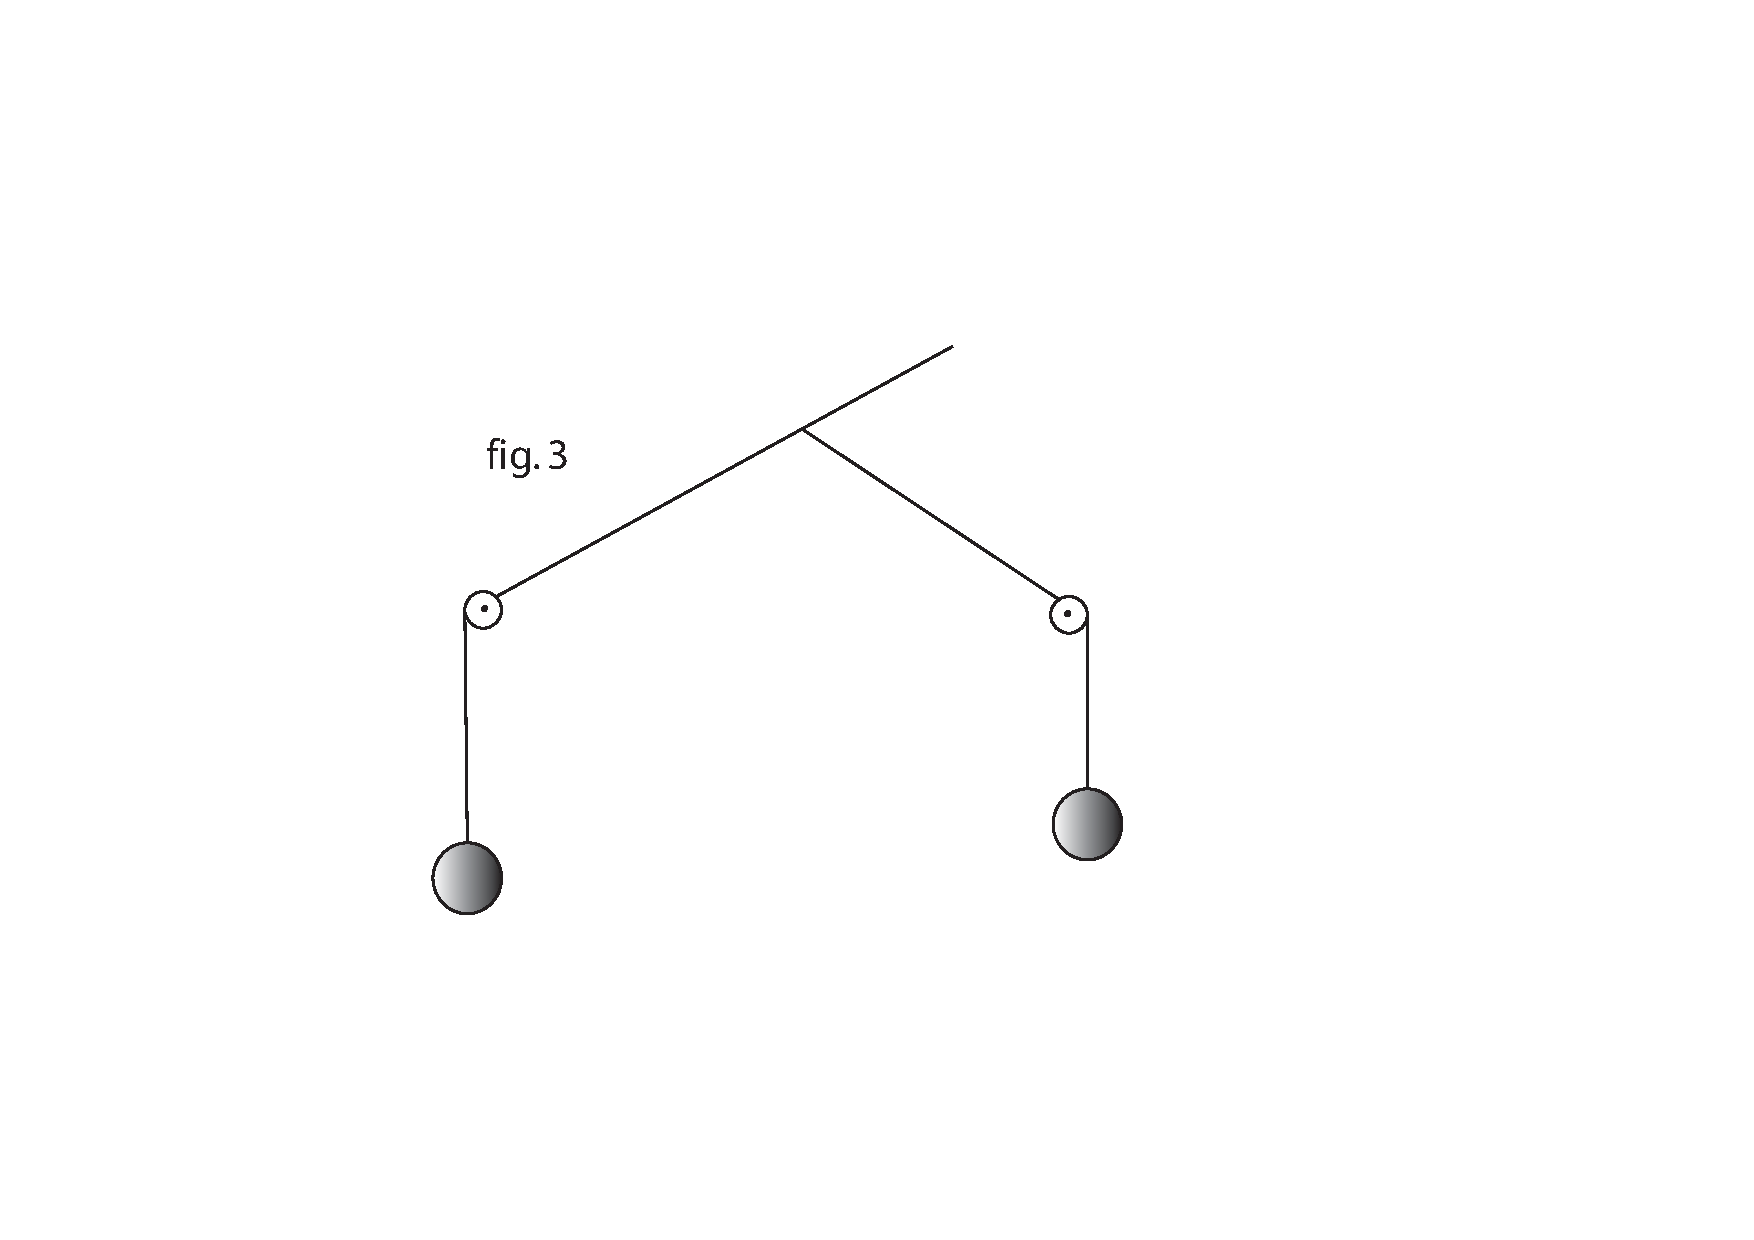
\includegraphics[width=0.43\textwidth]{images/LH03705_215r-d3.pdf}
\pend
\pstart%
\noindent%
\hangindent=7,5mm%
(6)\hspace{1mm}
\edtext{Locus Galilaei\protect\index{Namensregister}{\textso{Galilei} (Galilaeus, Galileus), Galileo 1564-1642}
contra quem P. Cazraeus\protect\index{Namensregister}{\textso{Le Cazre} (Cazreus), Pierre 1589-1664}
cum ratione disputavit.}{%
\lemma{Locus [...] disputavit}\Cfootnote{\cite{00050}\textsc{G. Galilei}, \textit{Discorsi}, Leiden 1638, S. 156ff., bes. S. 171-177 (\cite{00048}\textit{GO} VIII, S. 197ff., bes. S. 209-214).
\cite{01022}\textsc{P. le Cazre}, \textit{Physica demonstratio}, Paris 1645;
vgl. dazu \cite{00506}\textsc{A. Favaro}, \textit{Amici e corrispondenti di Galileo}, Flo\-renz 1983, Bd. III, S. 1531f.
Siehe hierüber N.~13.% Marginalien zu Le Cazre, Physica demonstratio.
}}
\pend
\pstart%
\noindent%
\hangindent=7,5mm
(7)\hspace{1mm}
\edtext{Lapsus Rohaultii Opticus.\protect\index{Namensregister}{Rohault, Jacques (1620-1675)}%
}{\lemma{Lapsus [...] Opticus}\Cfootnote{Vermut\-lich Anspielung auf die Ableitung der Gesetze der Lichtbrechung in \cite{00087}\textsc{J. Rohault}, \textit{Trait\'{e} de physique}, Teil I, Paris 1671, S. 116f. Sie hierzu \cite{01097}\textit{LSB} VIII, 1 N. 22.}}
\pend
\pstart%
\noindent%
\hangindent=7,5mm%
(8)\hspace{1mm}
\edtext{Paralogismus \textit{Geostaticae} Joh. Beaugrand,\protect\index{Namensregister}{\textso{Beaugrand}, Jean de 1595-1640}
et locus quo eum videtur confirmare Wallisius.\protect\index{Namensregister}{\textso{Wallis} (Wallisius), John 1616-1703}%
}{\lemma{Paralogismus [...] Wallisius}\Cfootnote{\cite{00334}\textsc{J. de Beaugrand}, \textit{Geostatice}, Paris 1636.
Siehe dazu N. 46. % Marginalien zu Beaugrand, Geostatice in VIII.2.
Anspielung auf Wallis nicht nachgewiesen.%
% \cite{00301}\textsc{J. Wallis}, \textit{Mechanica}, ??????, London 1670-1671, S. ??? (\cite{01008}\textit{WO} I, S. ???.)
}}
\pend
\count\Afootins=1500
\count\Bfootins=1500
\count\Cfootins=1500
%\pstart
%\centering
%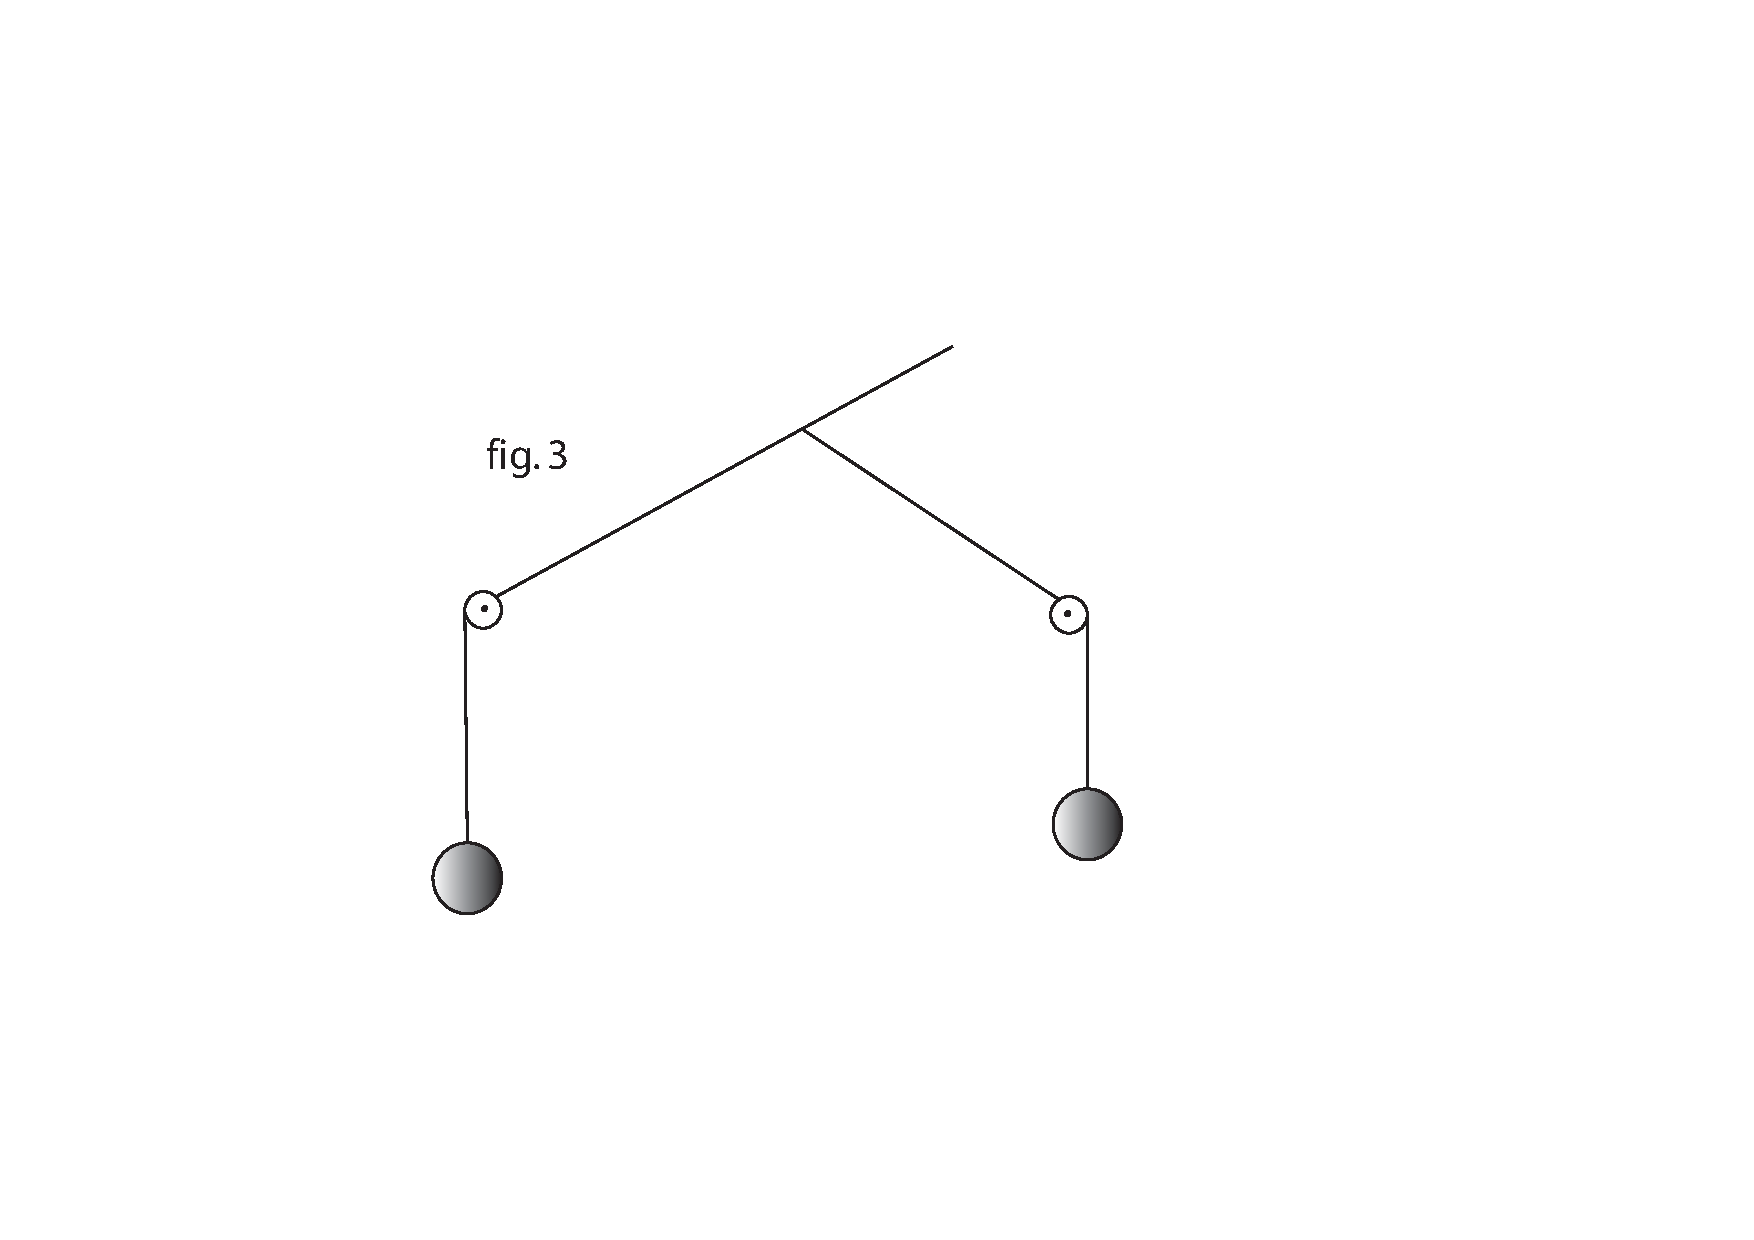
\includegraphics[width=0.4\textwidth]{images/LH03705_215r-d3.pdf}
%\pend
